\section{Diseño}
A continuación se presentan y explican algunas de las desiciones de diseño elegidas durante el desarrollo del trabajo practico.
Se decidió dividir la presentación en subsecciones para facilitar la comprensión de la misma, haciendo especial énfasis en aquéllas que consideramos son de mayor importancia para la comprensión del mismo.

%Vale mencionar que si bien es cierto que se genero una idea general en el grupo antes de comenzar a reflejar las decisiones tomadas en codigo, el diseño en profundidad se termino de desarrollar y afinar en paralelo, mientras surgian cuestiones mismas relacionadas al propio desarrollo que no habian sido tenidas en cuenta en papel. 


\subsection{Participantes, cap y fichas}
Decidimos que un en un modelado correcto del participante no tenía sentido desde el punto de vista de responsabilidades del objeto que lo represente que conozca su cap (presupuesto para armar equipos) ni su cantidad de fichas disponibles, puesto que no son esenciales. Por lo tanto, diseñamos dos clases, el GestorDeCap y el GestorDeFichas, cuyas instancias son objetos que conocen para un participante dado el cap y la cantidad de fichas disponibles respectivamente, además de proveer un protocolo para la actualización de esos valores, que nos permiten desligar a las instancias de la clase Participante de dichas responsabilidades.\\
El nombre Gestor para ambas clases proviene del hecho de que sus instancias gestionan las fichas/caps de los participantes, no són solo objetos que proveen información, sino que la mantienen también.\\
Instancias de ambas clases se utilizan también en la gestión de desafíos, dado que las apuestas afectan la cantidad de fichas disponibles de un participantes y el resultado de un desafíos afecta no sólo a las fichas disponibles de un participante, sino también a su cap.\\
El GestorDeCap entonces utiliza también la clase Presupuesto, que representa en el contextor del Gestor al presupuesto que un participante tiene como límite a la hora de conformar equipos.\\
Análogamente, el GestorDeFichas utiliza la clase Fichas, que representa una cantidad de fichas dada.\\
Si bien ambas clases parecen representar conceptos parecidos, preferimos organizar el conocimiento en dos clases distintas, para dejar en claro la diferencia existente entre ambas entidades en el dominio del problema.\\

\begin{center}
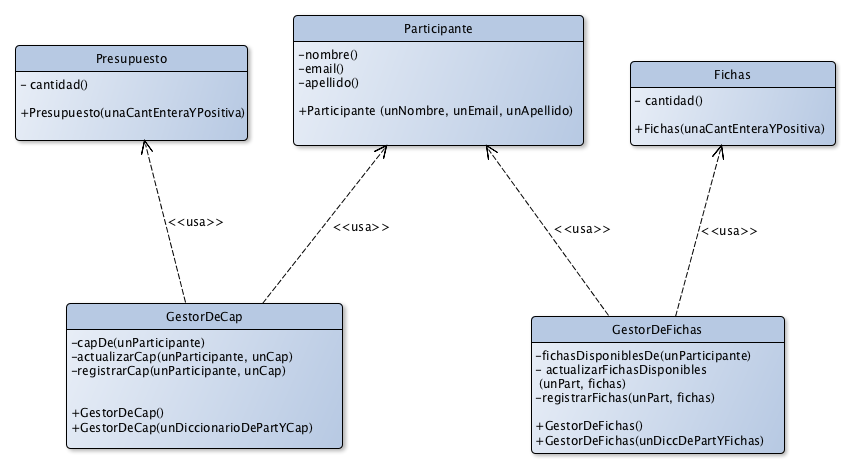
\includegraphics[scale=0.4]{diseno/gestorDeCapYFichas.png} 
\end{center}

Finalmente, con el mismo argumento esgrimido en párrafos anteriores, no es esencial al participante conocer directamente sus equipos. Resolvimos esto de una manera similar, como explicaremos en la siguiente subsección.\\


\subsection{Gestión de Equipos y Equipos}

\subsubsection{Gestor de Equipos}
Al no resultar esencial al participante conocer sus equipos, y no al no parecernos esencial al equipo conocer al participante, resolvimos diseñar una clase cuyas instancias proveen un protocolo para obtener los equipos de un participante, al igual que para crear, agregar y remover equipos para un participante dado.\\
Este objeto, además, es el encargado de realizar las validaciones correspondientes a la hora de registrar un equipo para un participantes. Es por esta razón que posee como colaboradores internos al GestorDeCap de la sección anterior (con el objetivo de no permitir la creación de equipos que superen el presupuesto de un participante), al igual que un objeto de la clase ListaPreciosJugador, encargado de conocer los precios de cada uno de los jugadores que viven en el modelo.\\
Esta última clases surgió también con un argumento similar a los expresados hasta ahora: no parecía ser ni esencial ni responsabilidad del jugador conocer su precio, sino que era un dato que se podría consultar a otra entidad.\\

\begin{center}
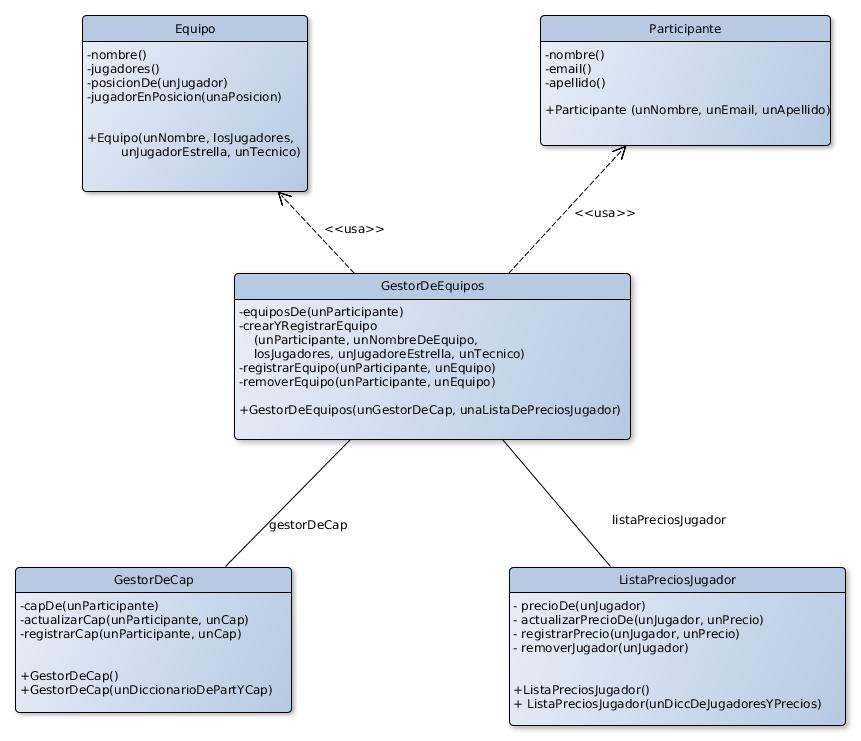
\includegraphics[scale=0.4]{diseno/gestorDeEquipos.jpg}
\end{center}

\subsubsection{Equipos}

Un equipo está conformado por sus cinco jugadores, uno de los cuales es un jugador estrella, y un técnico.
Lo primero a notar en nuestro modelado del equipo es que en realidad no debería ser esencial a un jugador su posición. La razón es simple: la posición en la que un jugador juega en un equipo es un componente estratégico, que incluso podría tener efectos a la hora de simular un partido. Por esta razón, es el equipo quien conoce la posición de un jugador dentro de sí mismo. Así, las instancias de la clases Equipo utilizarán las clases que subclasifican a la clase abstracta Posición. Modelar la posición con una jerarquía de clases cuyas instancias representarán los distintas posiciones nos permitirá que un equipo pueda responder con facilidad mensajes que devuelvan en qué posición juega un jugador en el equipo o qué jugador juega en el equipo en una posición dada, algo que resultó extremadamente útil a la hora de implementar la jugada defensiva Hombre a Hombre. Las posiciones y el equipo colaborarán en este caso en el contexto de un simulación haciendo uso del mecanismo de double dispatch, a fin de evitar la aparición de estructuras de control como if innecesariamente en el código fuente.\\
Además, de la misma manera en que no es responsabilidad de un jugador conocer su precio, tampoco lo es conocer sus estadísticas. Los objetos de la clase RegistroDeEstadisticas es quien conoce las estadísticas de los jugadores, como veremos en secciones subsiguientes.\\
Finalmente, un técnico conoce su nombre, su apellido, su nombre completo y su libro de jugadas de preferencia, esto último representado con instancias de la clase LibroDeJugadas, que hará uso de las clases JugadasOfensivas y JugadasDefensivas, a la vez que mantiene la frecuencia con la que se usa cada jugada, y que se usarán a la hora de elegir jugadas defensivas u ofensivas para el equipo según corresponda en el contexto de la simulación.\\
\begin{center}
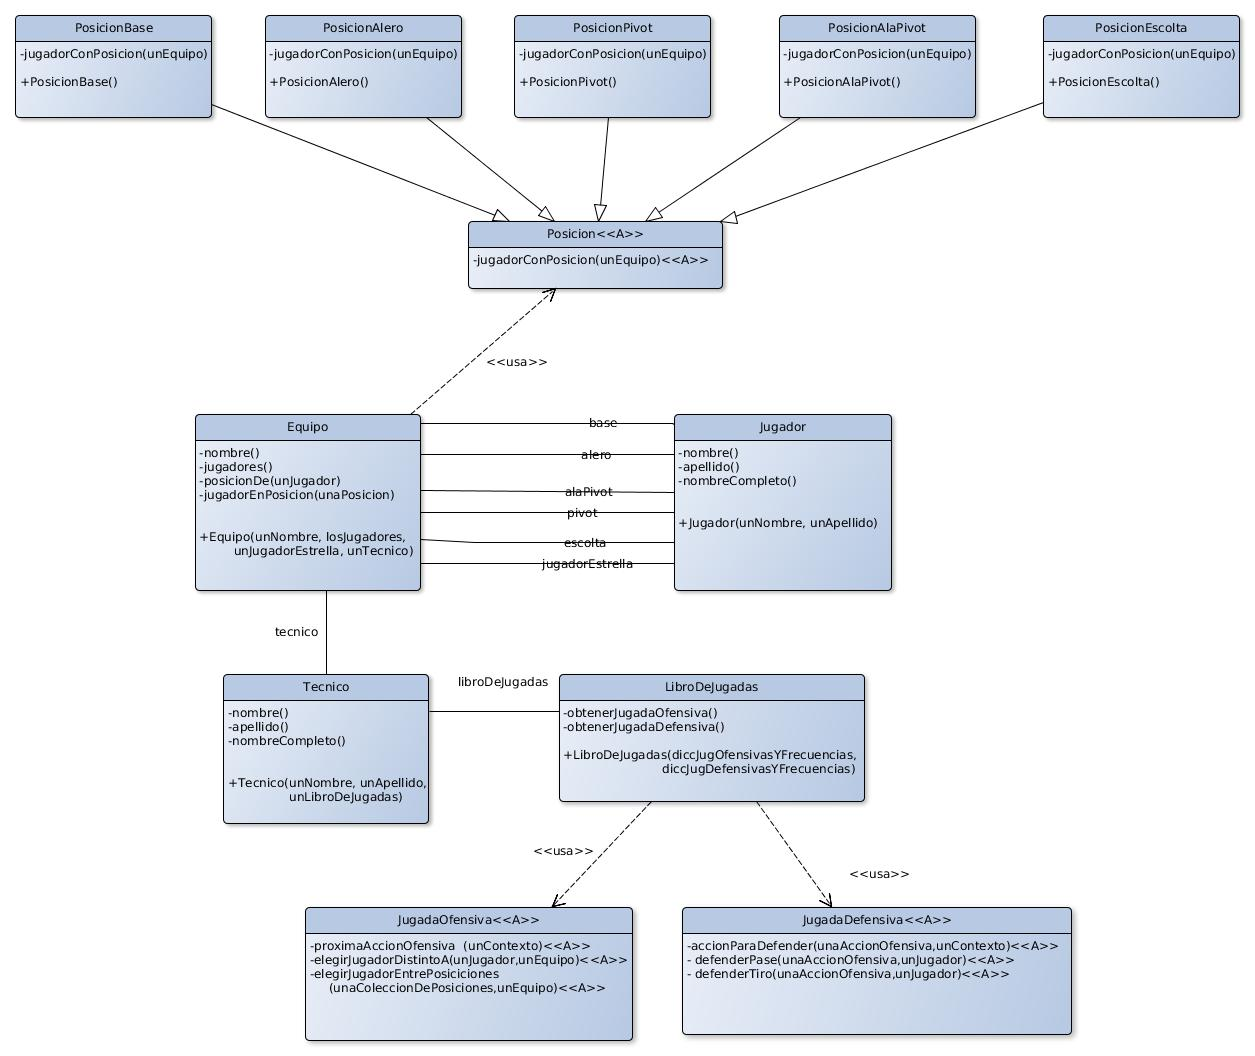
\includegraphics[scale=0.30]{diseno/equipo.jpg} 
\end{center}

\subsection{Registro de estadísticas}
Mencionamos en la sección anterior que no es responsabilidad de un jugador conocer sus estadísticas. Esta responsabilidad, entonces, recae en las instancias de la clase RegistroDeEstadísticas, que sabrán responder las estadísticas de un jugador dado, al igual que proveer un protocolo para actualizar las estadísticas de un jugador.\\
El nombre de Registro tiene sentido si le piensa como una entidad donde se pueden consultar y registrar las estadísticas de un jugador.\\
Para ello, además, modelamos a las estadísticas como instancias de la clase Estadística, que provee los mensajes necesarios para obtener las distintas estadísticas del jugador. Lo interesante de modelarla así es que en un futuro se podrán agregar nuevos tipos de estadísticas para el jugador de básquet: bastará con subclasificar la clase existente y definir los métodos a agregar.\\
\begin{center}
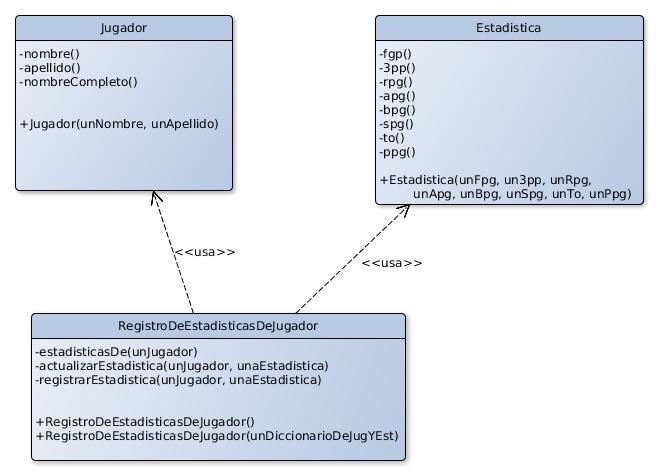
\includegraphics[scale=0.4]{diseno/registroDeEstadisticas.jpg}
\end{center}



\subsection{Acciones}

Diferenciamos principalmente dos tipos de acciones: las acciones ofensivas, como lo son los pases y los tiros al aro; y las defensivas, como el bloqueo y la intercepción.
Hay además una acción especial, el rebote, que se utiliza cuando al simular el reboteo durante un turno y que no es ni ofensiva ni defensiva.\\
Modelamos esto mediante la jerarquía de clases de Acciones. La clase abstracta Acciones define un protocolo abstracto de mensajes: jugadorEjecutante() y resolvedorPara(self). El primero viene a cuento de que en nuestro modelado de acciones, una acción conoce quién la va a ejecutar. Una acción colaborará con un simulador usando double dispatch para definir el resolvedor a usar para tal acción en el turno, que es el objeto que conoce las ecuaciones de resolución de las acciones.\\
La clase abstracta Accion se subclasifica entones en dos clases abstractas AccionOfensiva, AccionDefensiva y Rebote. A su vez, la AccionOfensiva se subclasifica en Pase (que además del ejecutante de la acción sabe responder el receptor del pase), Tiro2Puntos y Tiro3Puntos; y AccionDefensiva se subclasifica en Bloqueo e Intercepción.

\begin{center}
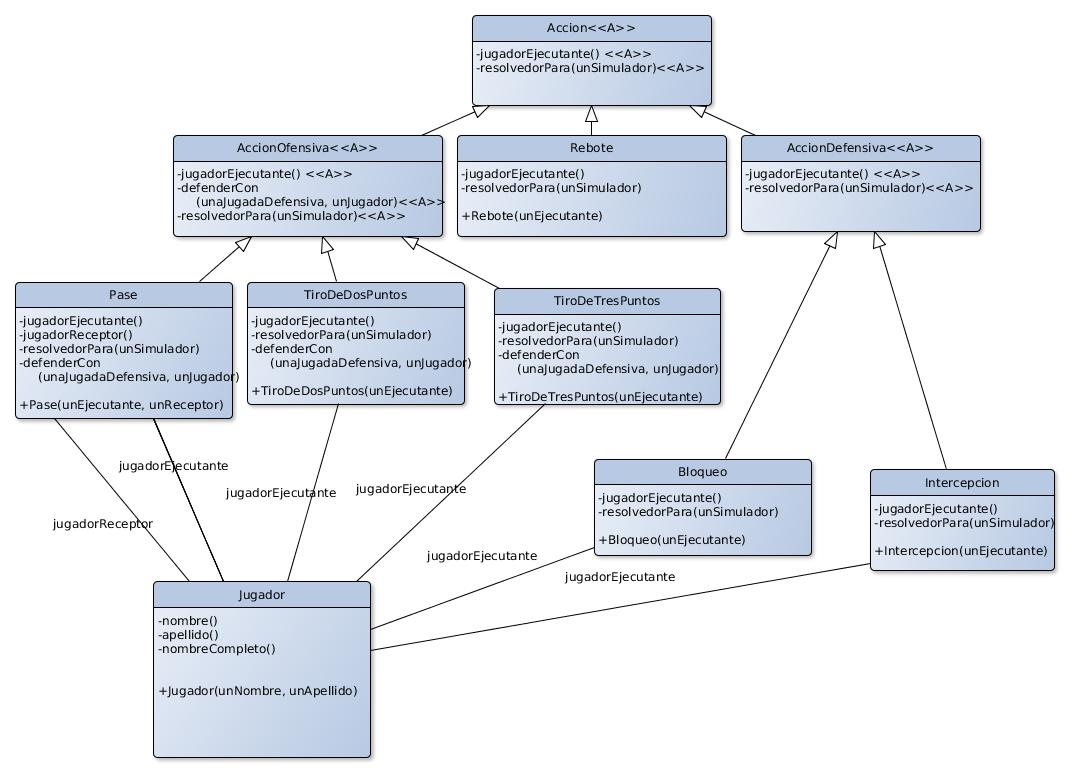
\includegraphics[scale=0.35]{diseno/acciones.jpg}
\end{center}

Mencionamos que un Simulador colabora con la acción para obtener un resolvedor, que conoce las reglas de resolución de las acciones. El siguiente diagrama de clases muestra la relación entre el Simulador y los distintos Resolvedores.


\begin{center}
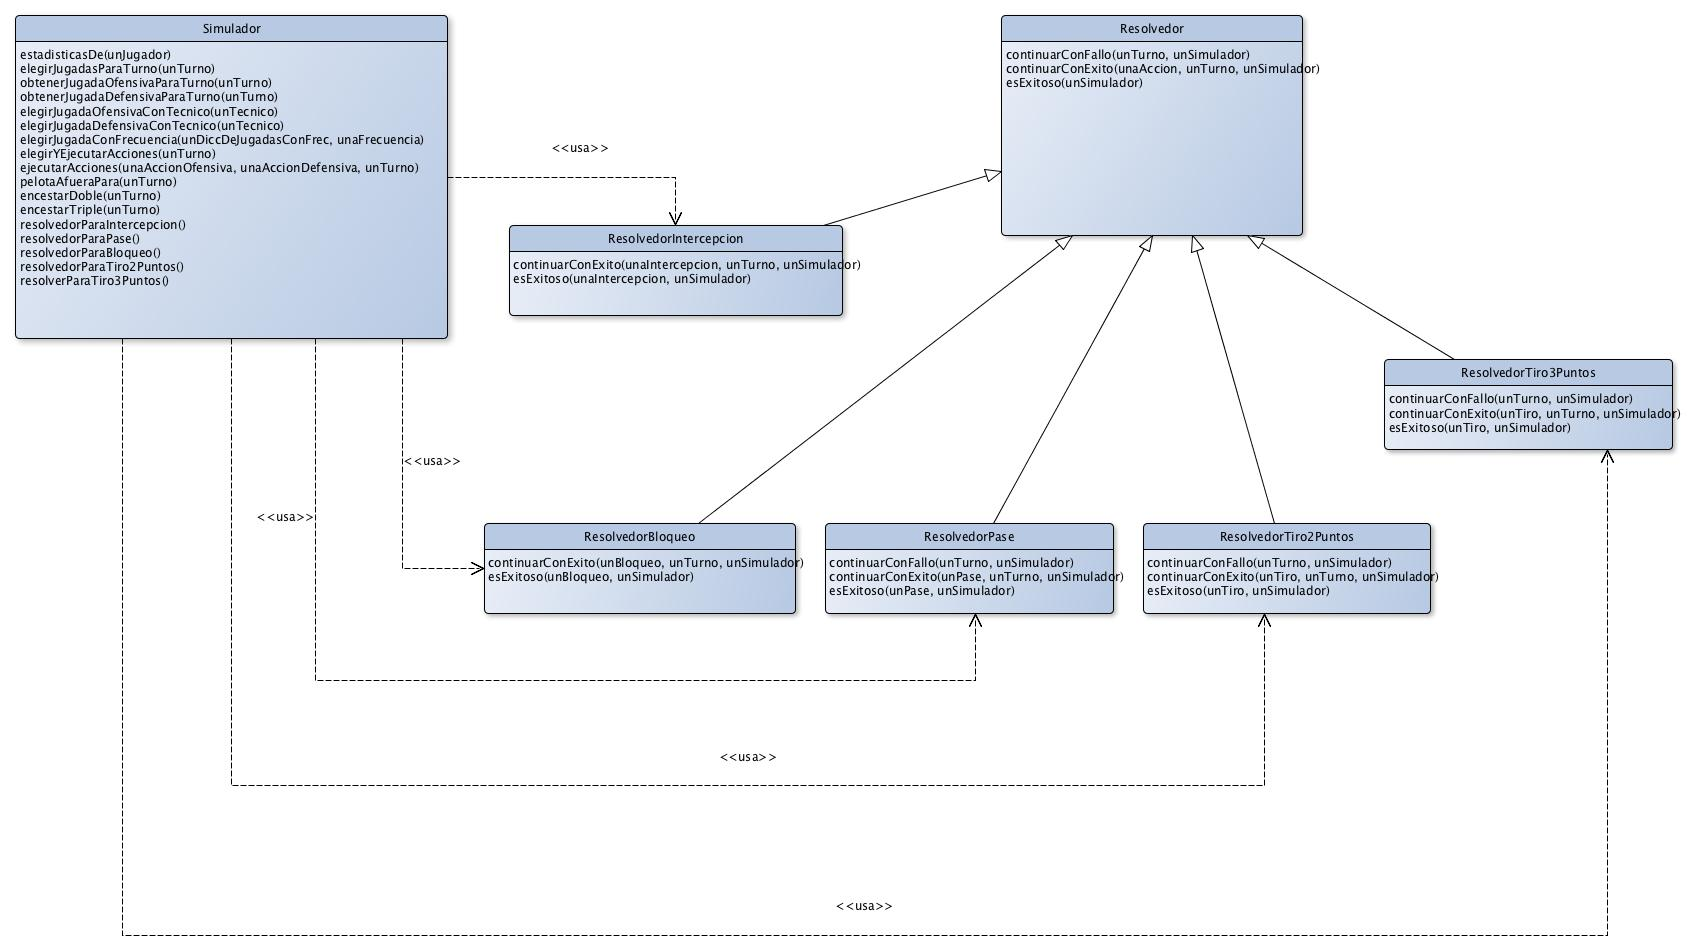
\includegraphics[scale=0.35, angle=90]{diseno/simuladorYResolvedor.jpg}
\end{center}

La clase abstracta Resolvedor representa a un resolvedor de acción, y conoce las reglas de resolución de la acción, al igual que hay acciones tomar en caso de éxito o fallo.\\
Se subclasifica a Resolvedor con Resolvedores concretos para cada una de las posibles acciones.
Dado que un resolvedor contiene las reglas de resolución de la acción, nos pareció lo más sensato que sean las instancias de la clase Simulador quiene usen las clases concretas de Resolvedor para obtener instancias.\\

La desventaja del enfoque utilizado para modelor esto, es que al agregar acciones necesitaremos agregar una nueva clase de resolvedor, además de modificar la clase Simulador (otra opción sería subclasificar Simulador con los métodos correspondientes para instanciar los nuevos resolvedores).\\


Veamos entonces como es que estas acciones se elijen y se ejecutan:
\begin{center}
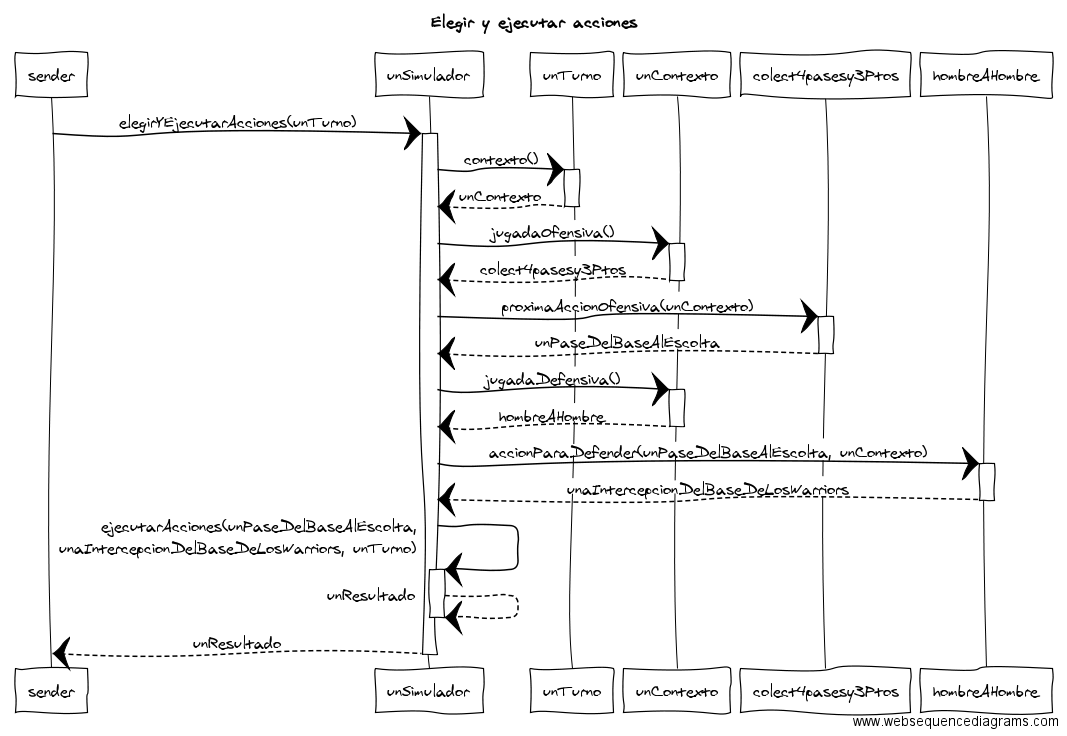
\includegraphics[scale=0.35]{diseno/Elegir_y_ejecutar_acciones.png}
\end{center}
Queda entonces claro como es que el simulador se encarga de tomar la jugada que se esta realizando del contexto y solicitarle las acciones correspondientes a cada una de estas para, luego de recibidas, proceder a ejecutarlas.

\subsection{Jugadas y acciones}
A continuación, presentamos entonces, como es que cada una de las acciones mencionadas en el apartado anterior, se integra con las jugadas defensivas/ofensivas, que componen los libros de los tecnicos.
\begin{center}
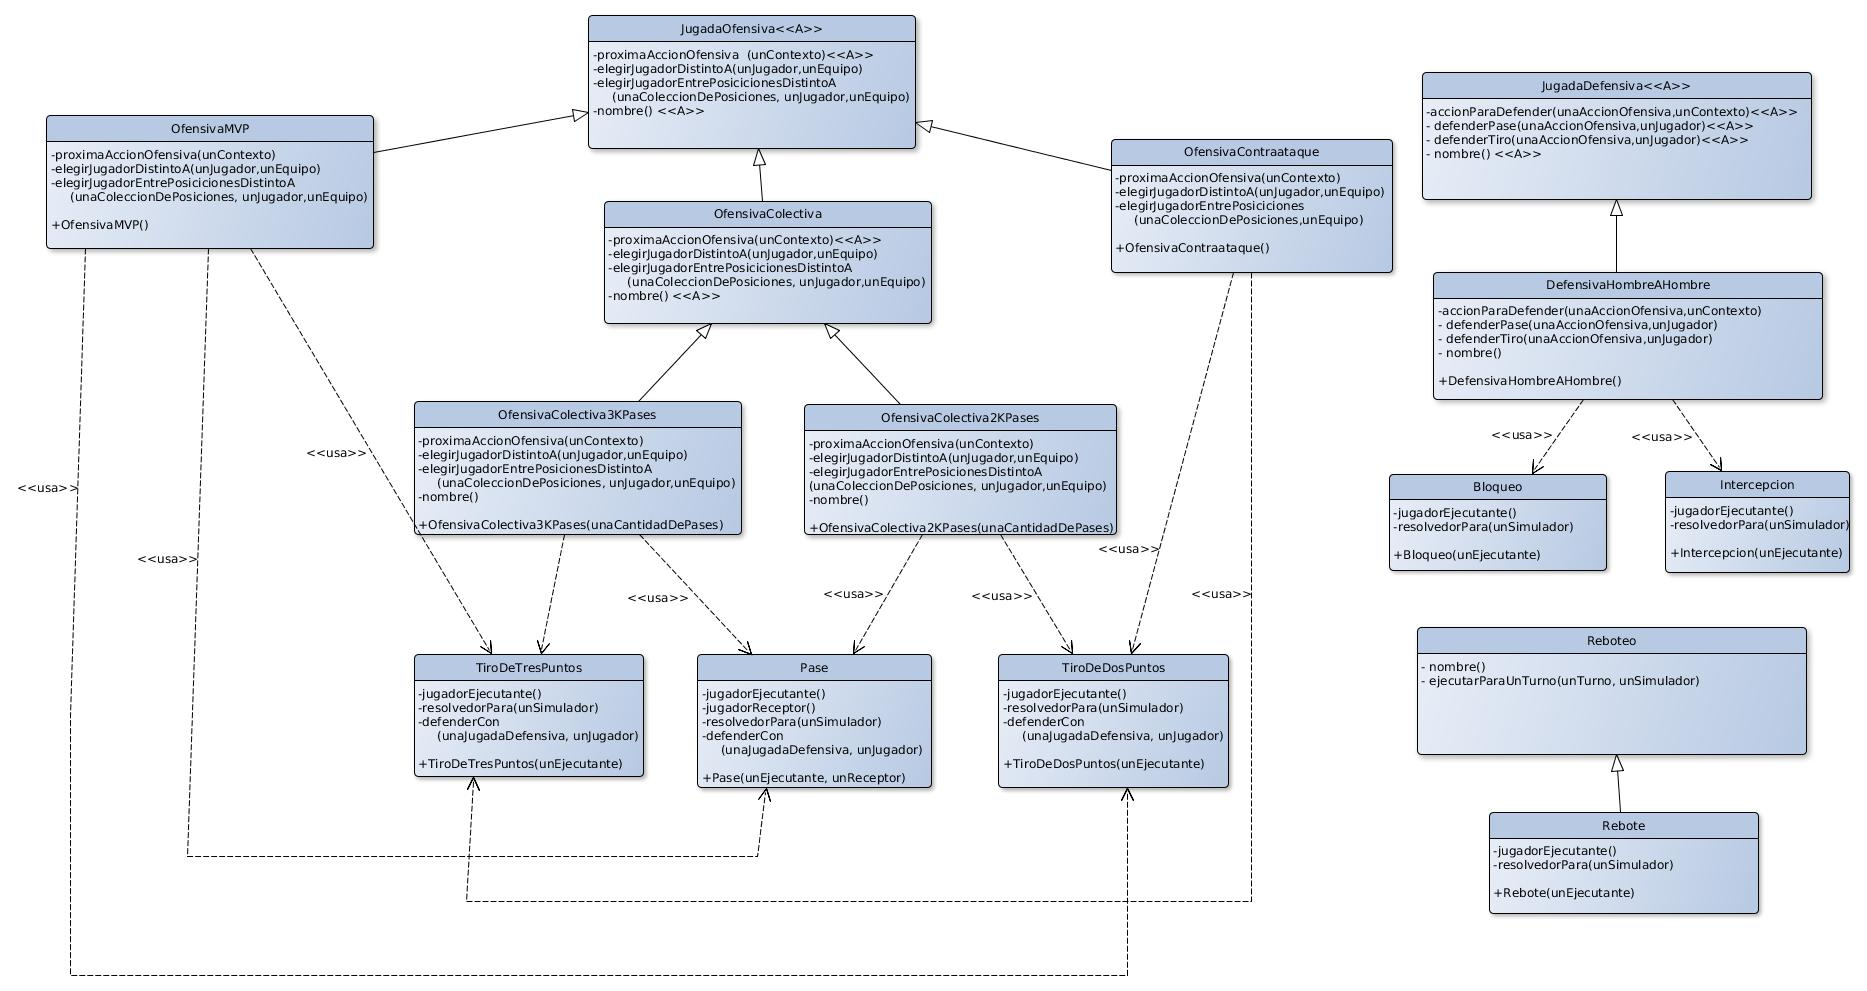
\includegraphics[scale=0.4, angle=90]{diseno/jugadasYAcciones.jpg}
\end{center}

En el siguiente diagrama de secuencia, podremos ver ademas, como estas distintas entidades encargadas de modelar las acciones de una jugada se relacionan con sus propios resolvedores. Estas ultimas son las entidades donde se calculan las distintas posibilidades de exito y fracaso para todas las interacciones entre dos jugadores. El hecho de que estos calculos no sean parte de las acciones en si, nos permite modificar los valores de las ecuaciones encargadas de calcular los resultados de cada accion de forma aislada y sin afectar al resto del modelo.

\begin{center}
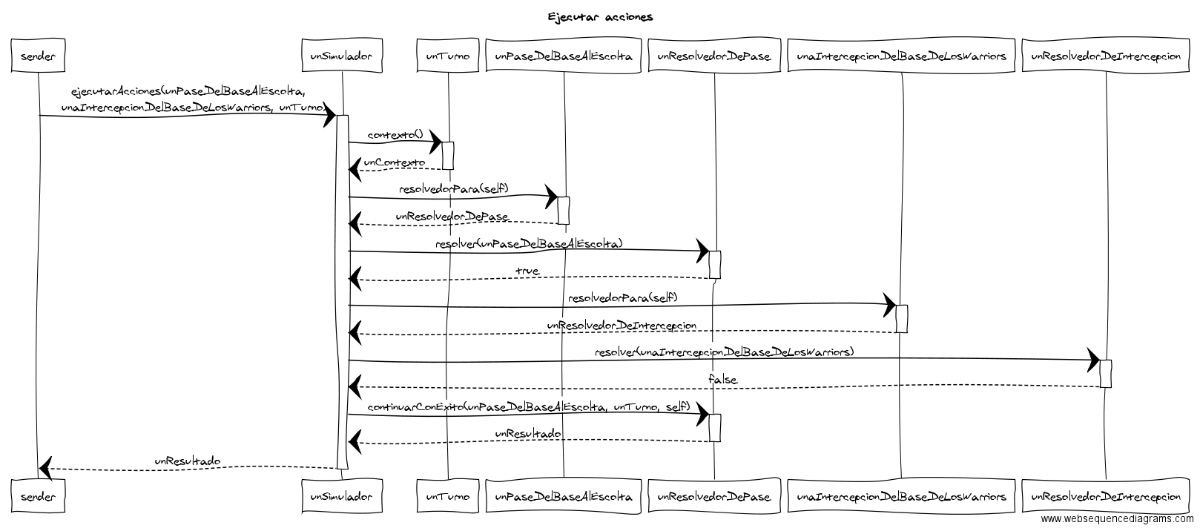
\includegraphics[scale=0.4, angle=90]{diseno/Ejecutar_acciones.png}
\end{center}


\subsection{Apuestas}
Decidimos que la mejor forma de clasificar las apuestas era mediante una jerarquizacion, para poder representar de forma clara que existen aquellas en las que se pone en juego un numero X de fichas, pero tambien aquellas nulas en las que no hay cap apostado. Esta clasificación, si bien es posible que agregue mas complejidad al diseño que suponiendo que las apuestas nulas son aquellas con cantidad de fichas igual a cero, nos ahorra de tener que manejar un unico tipo de apuesta y preguntar por la cantidad de fichas apostados todo el tiempo, permitiendo alijerar el manejo de las apuestas.
\begin{center}
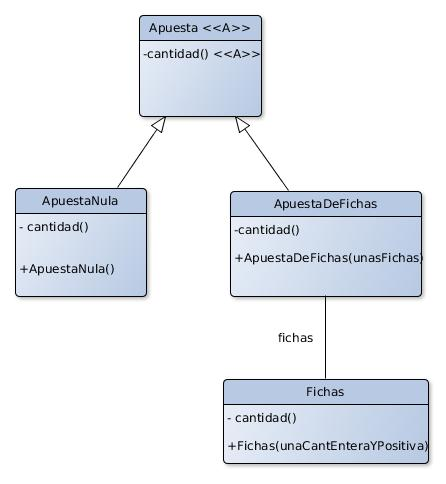
\includegraphics[scale=0.4]{diseno/apuestas.jpg}
\end{center}



A continuación veremos como se integran el tecnico con su libro de jugadas para elegir una jugada (en este caso, una ofensiva) con la simulación. Notese que, dado que las jugadas se eligen en base a la frecuencia de las mismas, se necesito de un generador de numeros aleatorios para simular el comportamiento de aleatoriedad en la eleccion de las mismas.
\begin{center}
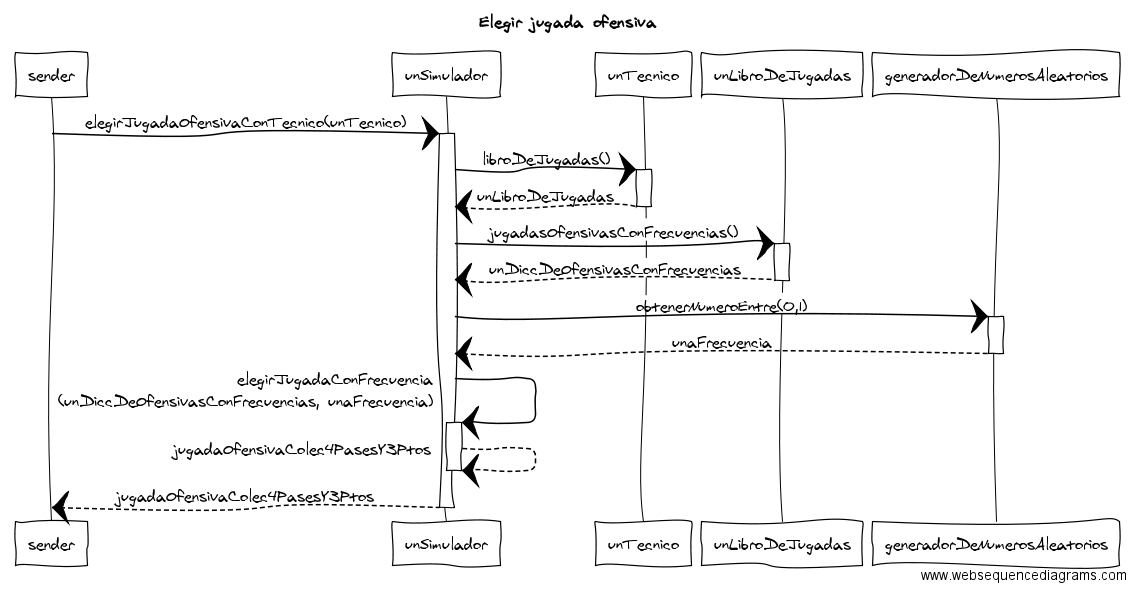
\includegraphics[scale=0.30]{diseno/Elegir_jugada_ofensiva.png} 
\end{center}


\subsection{Partido}
Analicemos ahora el diagrama de clases de las entidades que componen un partido podemos ver, en un planteo un poco mas general, como se realiza tambien el loggeo de las distintas acciones que realizan los jugadores y como se integra la entidad resultado para poder dar cuenta de como finalizan las distintas acciones que mencionamos en secciones anteriores. Todo el loggeo de las distintas acciones se realiza mediante una clase abstracta que permite que, en un futuro en lugar de imprimir la salida por consola como sucede actualmente, la forma de logear los resultados pueda ser alterada con un minimo impacto en el resto del sistema, disminuyendo la complejidad.
\begin{center}
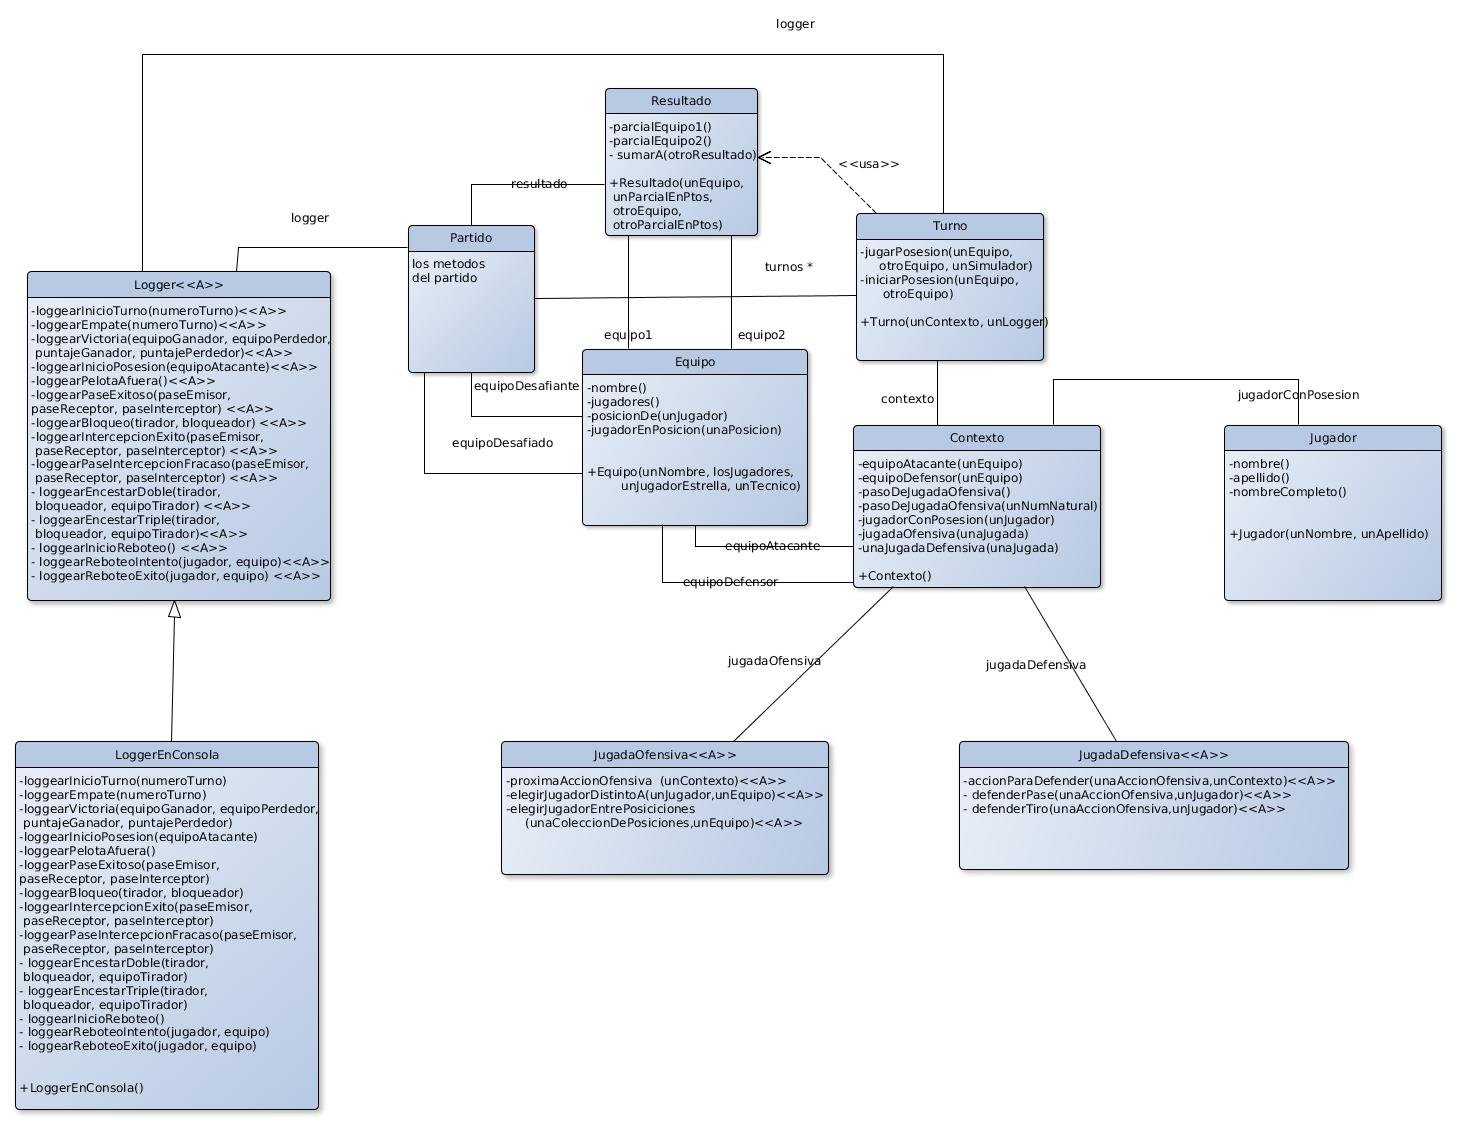
\includegraphics[scale=0.4, angle=90]{diseno/partido.jpg}
\end{center}

